\section{Derivations}
\label{app:derivations}

\subsection{Exact drift for general $K$ and estimators}
\label{app:drift}
Let $k$ be the number of $+$ answers among $K$ samples, $k\sim\mathrm{Bin}(K,p)$.
Given $k$ and the (tie-broken) majority $\hat a$, every sample with answer $c\in\{+,-\}$ receives the same reward $r_c=\mathbf 1[c=\hat a]$ and hence the same advantage $A_c$. The summed score-function gradient is $kA_+(1-p)-(K-k)A_-p$.
Averaging over tie-breaks gives coefficients $c_+(k)=\frac kK\mathbb E[A_+\mid k]$ and $c_-(k)=\frac{K-k}K\mathbb E[A_-\mid k]$, and
\begin{equation*}
  F(z)=\sum_{k=0}^K\binom Kk p^k(1-p)^{K-k}\,\big[c_+(k)(1-p)-c_-(k)p\big].
\end{equation*}
Write $\bar r=\max(k,K-k)/K$ for the mean reward when there is no tie. REINFORCE uses $A_c=r_c$, the mean baseline uses $A_c=r_c-\bar r$, and GRPO uses $A_c=(r_c-\bar r)/\sqrt{\bar r(1-\bar r)}$, with $A_c=0$ when all samples agree.
For $K=3$ the only non-degenerate configurations are the $2{:}1$ splits, where $\bar r=2/3$ and $\sqrt{\bar r(1-\bar r)}=\sqrt2/3$. The mean baseline therefore multiplies every contribution by $2/3$ and GRPO by $\sqrt2$, which proves the claim in \cref{sec:single}.
The same enumeration over multinomial count vectors gives the $M$-answer drift $g(z)\in\mathbb R^M$, whose components sum to zero.

\subsection{Linear stability and the amplification integral}
\label{app:stability}
Write $\epsilon=\eta t/N$ in \cref{eq:mf}.
Let the problems sit at $\pm a(t)$ with $da/d\epsilon=F(a)$, and let $w=\lambda v$ be a common logit shift.
Then $z_i=\pm a+w$ and $\langle F\rangle=\tfrac12[F(a+w)-F(a-w)]=F'(a)w+O(w^3)$, so
\begin{equation*}
  \frac{dw}{d\epsilon}=\lambda^2N\,F'(a)\,w\quad\Rightarrow\quad
  \ln\frac{w(\epsilon)}{w(0)}=\lambda^2N\int_0^\epsilon F'(a)\,d\epsilon'=\lambda^2N\ln\frac{F(a(\epsilon))}{F(a(0))}.
\end{equation*}
The amplification is largest at the window edge $a=z^\star$, which gives $\Lambda=\lambda^2N\ln[F^\star/F(a_0)]$.
After that point $F'<0$ and the shift is damped.
The per-problem term $\frac{\eta}{N}F'(z_i)$ in the full Jacobian amplifies differences between problems on the same side. This only reparametrizes time and cannot flip a problem.
The minority side flips once $w$ exceeds $a(t)$, which gives the threshold $\Lambda\approx\ln(1/\delta)+O(1)$.

For a heterogeneous population, each problem follows $dz_i/d\epsilon=F(z_i)$ to leading order, and the shift grows at rate $\lambda^2N\langle F'(z(\epsilon))\rangle$. The maximal log-amplification is therefore $\lambda^2N\sup_\epsilon\int_0^\epsilon\langle F'\rangle d\epsilon'$.

\subsection{Size of the noise seed}
\label{app:seed}
With minibatches of $B$ problems and step $\eta$, the shared shift receives zero-mean noise of standard deviation $\eta\lambda^2\sigma/\sqrt B$ per step, where $\sigma^2$ is the variance of the single-problem gradient estimate.
Noise injected within the first growth time $t_{\rm g}=1/(\eta\lambda^2F'(a))$ is amplified almost fully, which gives an effective seed $\delta^2\simeq t_{\rm g}\,\eta^2\lambda^4\sigma^2/B=\eta\lambda^2\sigma^2/(BF'(a))$ and $\ln(1/\delta)=\tfrac12\ln B+\ln(1/\lambda)-\tfrac12\ln\eta+\text{const}$.
Under the linear scaling rule $\eta\propto B$ the dependence on $B$ cancels.

\subsection{Mean-field check of the closed form}
\label{app:mfcheck}
We check \cref{eq:Nc} in the noise-free limit, where it can be tested exactly.
In rescaled time $s=\eta t/N$, the deterministic two-population version of \cref{eq:mf} reads $dz_\pm/ds=F(z_\pm)+\lambda^2N\langle F\rangle$, where $z_+$ and $z_-$ are the logits of the problems that start at $+a$ and $-a$ (without sampling noise, all problems in each group stay identical) and $\langle F\rangle=\tfrac12[F(z_+)+F(z_-)]$. It depends on $\lambda$ and $N$ only through $X=\lambda^2N$, so in mean field $N_c\propto\lambda^{-2}$ holds exactly.
Solving for the critical $X_c(a,\delta)$ by bisection, the exact critical amplification $X_cG(a)$ equals $\ln(1/\delta)-c$, with unit slope in $\ln(1/\delta)$ over $\delta\in[10^{-6},10^{-2}]$ and a weakly $a$-dependent offset $c\in[0.9,2.0]$ for $a\in[0.3,1.25]$ ($c\approx1.1$ at $a=0.5$; \cref{tab:mf}). This is the form asserted by \cref{eq:Nc}.
The constant offset is the $O(1)$ threshold $w\sim a$ required for the minority side to flip.
In the stochastic simulations of \cref{sec:sims} we measure $\Lambda_c\approx2.6$ at $a=0.5$ (\cref{fig:scaling}b). Inverting $\Lambda_c=\ln(1/\delta_{\rm eff})-c$ with $c\approx1.1$ gives an effective noise seed $\delta_{\rm eff}\approx e^{-3.7}\approx0.02$.

\begin{table}[h]
\centering\small
\caption{Deterministic mean-field critical amplification $X_cG(a)$ (with $X=\lambda^2N$) against the closed-form prediction $\ln(1/\delta)$.}
\label{tab:mf}
\begin{tabular}{lcccc}
\toprule
$a$ & $\delta=10^{-2}$ & $\delta=10^{-3}$ & $\delta=10^{-4}$ & $\delta=10^{-6}$ \\
\midrule
0.1 & 2.25 & 4.50 & 6.77 & 11.32 \\
0.3 & 3.23 & 5.47 & 7.72 & 12.26 \\
0.5 & 3.60 & 5.83 & 8.07 & 12.59 \\
0.8 & 3.75 & 5.96 & 8.19 & 12.70 \\
1.1 & 3.50 & 5.69 & 7.92 & 12.41 \\
1.25 & 2.99 & 5.16 & 7.38 & 11.85 \\
\midrule
$\ln(1/\delta)$ & 4.61 & 6.91 & 9.21 & 13.82 \\
\bottomrule
\end{tabular}
\end{table}


\subsection{Many answers}
\label{app:multi}
Let $z_i=a\,e_{s_i}$ with labels $s_i$ balanced over $\{1,\dots,M\}$, and let $w=\lambda v\in\mathbb R^M$.
Then $\dot w=\eta\lambda^2\langle g(z_i+w)\rangle$, whose linearization is $\eta\lambda^2\bar J w$ with $\bar J=\frac1M\sum_s\partial g/\partial z\,|_{ae_s}$.
Averaging over $s$ makes $\bar J$ permutation-invariant, so on the zero-sum subspace (the only identifiable directions under softmax) $\bar J=\kappa(a)I$ with $\kappa=\mathrm{tr}(P\bar JP)/(M-1)$ and $P=I-\frac1M\mathbf1\mathbf1^\top$.
The margin $a$ between the preferred and the other logits obeys $\dot a=\frac\eta N f(a)$ with $f=g_{s}-g_{\neq s}$.
Dividing the two rates gives $\Lambda=\lambda^2N\int_{a_0}^{a^\star}\kappa/f\,da$.
For $M=2$ this reduces exactly to the binary result; we checked this numerically.

\subsection{Kernel form}
\label{app:kernel}
In a linearized network, $\dot z=\frac\eta N\mathbf K F(z)$.
Take $\mathbf K=k_d'\mathbf I+k_u\mathbf1\mathbf1^\top+k_sss^\top$ with balanced signs $s$, so that $\mathbf1\perp s$, and a homogeneous population $z_i=s_ia$.
Then $\dot z_i=\frac\eta N(k_d'+Nk_s)F(a)s_i$, so $\dot a=\frac\eta N(k_d'+Nk_s)F(a)$: sharpening is accelerated by the prediction-aligned coupling.
A common shift $z_i=s_ia+w$ gives $F(z_i)=s_iF(a)+F'(a)w+O(w^2)$, since $F$ is odd and $F'$ even. With $\mathbf K\mathbf1=(k_d'+Nk_u)\mathbf1$ this gives $\dot w=\frac\eta N(k_d'+Nk_u)F'(a)w$.
Dividing by $\dot a$ eliminates time:
\begin{equation*}
  \frac{d\ln w}{da}=\frac{k_d'+Nk_u}{k_d'+Nk_s}\,\frac{F'(a)}{F(a)}.
\end{equation*}
Integrating from $a_0$ to $z^\star$ gives
\begin{equation*}
  \Lambda=G(a_0)\,\frac{Nk_u}{k_d'+Nk_s}+G(a_0)\,\frac{k_d'}{k_d'+Nk_s}.
\end{equation*}
The second term is the self-term. It is at most $G$ and independent of $N$, and it is the growth that remains with the coupling switched off, when each problem follows its own sign-preserving flow and cannot flip. It is therefore absorbed into the $O(1)$ of the threshold, as in the toy model (\cref{app:stability}), and dropping it gives \cref{eq:kernel}. The $k_d'$ in the denominator sets the sharpening rate and multiplies the leading term, so it is kept.
We estimate $k_d$ as the mean diagonal of the empirical kernel, $k_u$ as the mean off-diagonal, and $k_s$ as the mean off-diagonal of $s_is_j\mathbf K_{ij}$, and set $k_d'=k_d-k_u-k_s$.

\paragraph{Kernel mean-field predictor.}
The deterministic baseline of \cref{sec:nn} integrates the projected dynamics directly. Writing $\epsilon=\eta k_d't/N$ and $\langle sF\rangle=\frac1N\sum_js_jF(z_j)$,
\begin{equation*}
  \frac{dz_i}{d\epsilon}=F(z_i)+\frac{Nk_s}{k_d'}\,s_i\langle sF\rangle+\frac{Nk_u}{k_d'}\,\langle F\rangle,
\end{equation*}
integrated from the measured initial logits over the same training horizon as the RL runs.

\subsection{Marginal-entropy remedy}
\label{app:remedy}
The bonus $\beta H(\bar p)$ adds $\beta\ln\frac{1-\bar p}{\bar p}\,p_i(1-p_i)$ to the gradient on $z_i$.
For a common shift $w$, $\bar p-\tfrac12\approx\langle p(1-p)\rangle w$ and $\ln\frac{1-\bar p}{\bar p}\approx-4(\bar p-\tfrac12)$.
Averaging over problems shows that the shared-mode growth rate becomes $\eta\lambda^2(\langle F'\rangle-4\beta\langle p(1-p)\rangle^2)$, which gives \cref{eq:beta}.
At $z=0$, $F'(0)=1/8$ and $p(1-p)=1/4$, so $\beta_c=1/2$, the maximum over $a$.


% ---------------------------------------------------------------------------
\section{Further Results for the Solvable Model}
\label{app:simdetails}
This section collects the numbers behind \cref{sec:sims}.

\subsection{Fitted critical sizes (P1, P2)}
\label{app:fits}
The default settings are REINFORCE, $K{=}3$, $B{=}32$, SGD with step $\eta{=}4$ and 300 epochs, so each visit changes $u_i$ by $(\eta/B)\,\hat g_i=0.125\,\hat g_i$. Each configuration is run with 16--24 seeds.
In collapsing runs the self-assessed reward goes to $0.999$ while accuracy falls from $0.80$ to $0.50$ (\cref{fig:mechanism}b). Near $N_c$ the outcome is fixed within the first ${\sim}100$ epochs (\cref{fig:mechanism}c), and the probability of collapse rises from $0$ to $1$ within a factor of about $3$--$4$ in $N$ (\cref{fig:scaling}a).
Varying only the coupling, $\lambda\in[0.035,0.28]$, moves the critical size from $N_c=5750$ to $N_c=60$, and a power-law fit gives $N_c\propto\lambda^{-2.22}$ (\cref{fig:scaling}c).
Varying only the initial confidence, $a\in[0.15,1.1]$, moves $N_c$ from $189$ to $8740$ (\cref{fig:scaling}d).
The fitted critical amplification is $\Lambda_c=2.64$, and the twelve sweeps (seven couplings and five confidences) give values in $[2.1,3.6]$ (\cref{fig:scaling}b).


\begin{figure}[t]
\centering
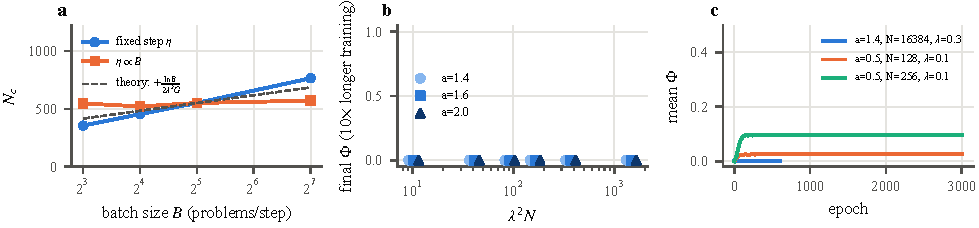
\includegraphics[width=\textwidth]{../figures/fig_batch_stable.pdf}
\caption{\textbf{Batch size and long training.} (a)~$N_c$ against batch size, with a fixed step (blue) and with linear step scaling (orange). The dashed line is the logarithmic prediction anchored at $B{=}32$. (b)~Final order parameter after $10\times$ longer training for confident initial models ($a>z^\star$) at values of $\lambda^2N$ up to $1474$. Uncertain models collapse for $\lambda^2N\gtrsim5$. (c)~Order-parameter trajectories: confident models stay balanced, and sub-critical uncertain models remain balanced after sharpening.}
\label{fig:batch}
\end{figure}

\subsection{Batch size enters logarithmically (P3)}
\label{app:batch}
The remaining input to \cref{eq:Nc} is the noise seed $\delta$, which the batch size controls.
With a fixed step size, a $16\times$ change in batch size ($B=8\to128$) changes $N_c$ by only $2.2\times$ ($355\to765$, \cref{fig:batch}a), roughly linearly in $\ln B$ as predicted. The crude seed estimate in \cref{app:derivations} gives a slope of $0.5/(\lambda^2G)$ per unit $\ln B$; we measure about $1.5\times$ that.
For $B=512$ every tested size ($N\ge2B$) already collapses, consistent with $N_c<1024$.
Under the linear scaling rule $\eta\propto B$, which keeps the noise per sample fixed, $N_c$ is flat ($521$--$572$ for $B=8$--$128$, orange in \cref{fig:batch}a), again as predicted by \cref{app:seed}.
At $B=512$ with linear scaling the step on the shared parameter ($\eta\lambda^2=0.64$) is too large for the small-step approximation, and all runs collapse.
For comparison, a $16\times$ change in $\lambda^{-2}$ moves $N_c$ by $18$--$26\times$ (\cref{fig:scaling}c).

\subsection{Confident models are stable, not merely slow (P4)}
\label{app:stable}
The last prediction concerns models that start outside the unstable window, which the theory says are stable rather than merely slow to collapse.
To distinguish stability from slow dynamics, we train confident models, $a\in\{1.4,1.6,2.0\}>z^\star$, at couplings and sizes far beyond the uncertain-model threshold: up to $\lambda^2N=1474$, where an $a=0.5$ population would reach $\Lambda\approx760$.
For $N=1024$ and $4096$ we train $10\times$ longer (3000 epochs), and for $N=16384$ $2\times$ longer.
Across all 18 configurations (16 seeds each) \emph{not a single problem flips} its answer. The shared shift stays at $|\lambda v|\le0.013$, and accuracy stays at its initial $0.80$ (\cref{fig:batch}b,c).
Sub-critical uncertain models ($a=0.5$, $N\le256$, $\lambda^2N\le2.6$) also remain uncollapsed under $10\times$ longer training ($\Phi\le0.1$ on average, \cref{fig:batch}c).
Once the population has left the unstable window, the shared mode is damped, so training longer does not lead to collapse.

\subsection{Heterogeneity, feature coupling and remedy}
\label{app:hetero}
\paragraph{Heterogeneous confidence.}
We draw $|z_i(0)|$ from seven distributions: uniform on $[0,1]$, $[0,2]$, $[0,3]$ and $[0.5,2.5]$; exponential with mean $0.7$; and two-point mixtures with $30\%$ or $60\%$ of problems at $0.3$ and the rest at $2.0$.
For each we compute $G[\rho_0]$ from the initial distribution alone, using its definition in \cref{sec:general}.
The measured $N_c$ spans $455$--$14{,}700$, and $\Lambda_c\in[2.0,2.8]$ throughout (\cref{fig:hetero}a).
In the 30\% mixture most problems are confident, yet the population still collapses, at $N_c\approx14{,}700$, consistent with its small but positive $G=0.014$.
For the uniform $[0.5,2.5]$ population, $\langle F'\rangle<0$ from the start, so $G=0$, and no run collapses even at $N=24{,}000$.

\paragraph{Feature coupling.}
We add a coupling $z_i\mathrel{+}=\mu s_iw$ aligned with each problem's initial preference $s_i$. The kernel theory (\cref{eq:kernel}) predicts $N_c=1/(\lambda^2G/\Lambda_c-\mu^2)$, which diverges at $\mu_c=\sqrt{\lambda^2G/\Lambda_c}$. With $\lambda=0.1$, $G(0.5)=0.514$ and $\Lambda_c=2.64$ this gives $\mu_c=0.044$.
The transition broadens near the divergence (\cref{fig:hetero}b). For $\mu=0.04$ only $44\%$ of runs collapse even at $N=32768$, and for $\mu\ge0.05$ no run collapses at any $N$ up to $32768$.

\paragraph{Marginal-entropy remedy.}
\Cref{eq:beta} gives $\beta_c(0.2)=0.49$ and $\beta_c(0.5)=0.44$.
At $\beta=0.5$ and above, no run collapses for any $N\le8192$ or either $a$, and accuracy stays at its sharpening-only value ($0.78$ for $a=0.5$). At $\beta=0.25$, runs survive at $N=512$ but collapse at $N=8192$ (\cref{fig:hetero}c).
At $\beta\ge\beta_c$ the final confidence $\langle|z|\rangle$ is the same as in sub-critical runs without the bonus.

% ---------------------------------------------------------------------------
\section{Robustness: GRPO, Group Size, Many Answers, Adam}
\label{sec:robust}

All discussions in the main text use one training setup: REINFORCE with $K=3$, binary answers and plain SGD. Here we vary each of these choices, still in the toy model, to check that the law of \cref{sec:theory} is not an artifact of the defaults.

\begin{figure}[t]
\centering
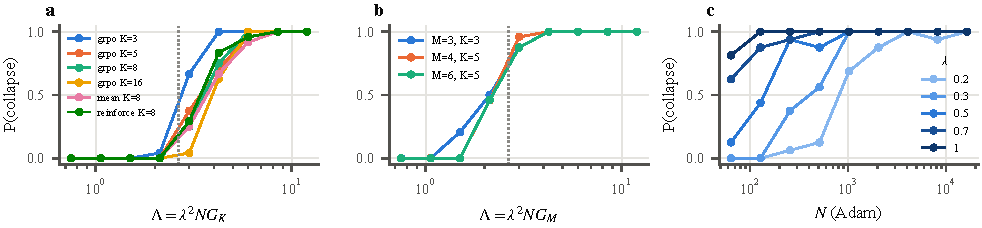
\includegraphics[width=\textwidth]{../figures/fig_robust.pdf}
\caption{\textbf{Robustness.} (a)~GRPO and REINFORCE for $K\in\{3,5,8,16\}$ against $\Lambda=\lambda^2NG_K$, where $G_K$ (\cref{sec:race}) is computed from the exact $K$-sample drift $F_K$ (\cref{sec:single}). (b)~$M$-answer softmax policies against $\Lambda=\lambda^2NG_M$. (c)~Adam: probability of collapse against $N$ for several couplings.}
\label{fig:robust}
\end{figure}

\begin{table}[h]
\caption{Edge of the unstable window $z^\star_K$ (where $F_K'=0$) and the amplification factor $G_K(0.5)=\ln[F^\star_K/F_K(0.5)]$ for different estimators and group sizes $K$ (binary answers). Computed exactly by enumeration.}
\label{tab:window}
\centering\small
\begin{tabular}{lccccc}
\toprule
 & $K=3$ & $4$ & $5$ & $8$ & $16$ \\
\midrule
\multicolumn{6}{l}{\emph{REINFORCE:} $z^\star_K$} \\
 & 1.317 & 1.274 & 1.187 & 1.088 & 0.894 \\
\multicolumn{6}{l}{\emph{GRPO (std-normalized):} $z^\star_K$} \\
 & 1.317 & 1.317 & 1.213 & 1.172 & 1.006 \\
\midrule
\multicolumn{6}{l}{\emph{REINFORCE:} $G_K(0.5)$} \\
 & 0.514 & 0.484 & 0.426 & 0.353 & 0.202 \\
\multicolumn{6}{l}{\emph{GRPO:} $G_K(0.5)$} \\
 & 0.514 & 0.514 & 0.443 & 0.408 & 0.258 \\
\bottomrule
\end{tabular}
\end{table}

\paragraph{GRPO and group size.}
For $K=3$, GRPO's drift is exactly $\sqrt2F$ (\cref{sec:single}). The constant factor cancels in $G$, so $G_3(0.5)=0.514$ for both estimators (\cref{tab:window}), and the theory predicts the same $N_c$.
The simulations agree: the logistic fit to the GRPO $K=3$ curve in \cref{fig:robust}a gives $N_c=548$, against $N_c=536$ for REINFORCE at the same $\lambda=0.1$ and $a=0.5$ (\cref{fig:scaling}c).
Larger groups have smaller $G_K$ (\cref{tab:window}), so the theory predicts larger $N_c$. The fitted values rise to $793$, $876$ and $1557$ for $K=5,8,16$ (\cref{fig:robust}a), in the order predicted by $G_K$.
Computing $\Lambda_c=\lambda^2N_cG_K$ from these fits, the critical amplification drifts mildly upward with $K$ ($\Lambda_c=2.8\to4.0$), consistent with the smaller gradient noise and hence smaller seed $\delta$ of larger groups.
The mean baseline and REINFORCE at $K=8$, also shown in \cref{fig:robust}a, give $\Lambda_c=3.8$ and $3.5$, within this band.

\paragraph{Many answers.}
Next we replace binary answers by $M$-answer softmax policies, as in the theory of \cref{sec:general}.
With $M\in\{3,4,6\}$ answers, softmax logits and a shared bias \emph{vector}, the collapsed state has every problem giving the same answer, and accuracy drops to $1/M$.
Using the eigenvalue-based $G_M$ of \cref{sec:general}, computed by exact enumeration (\cref{app:multi}), the transitions fall at $\Lambda_c=2.1$--$2.2$ (\cref{fig:robust}b), slightly below the binary value. This is consistent with $M-1$ noisy shared directions seeding the instability.

\paragraph{Adam.}
The last change is the optimizer. Unlike the changes above, it alters the rates in the theory itself, so we first rederive the scaling.
Adam \citep{kingma2015adam} normalizes each coordinate by its own gradient scale, which changes both rates in the race.
The shared parameter sees a gradient dominated by noise of scale $\lambda\sigma/\sqrt B$, so its signal-to-noise-normalized drift makes the shared mode grow at a rate $\propto\lambda\langle F'\rangle$ rather than $\lambda^2\langle F'\rangle$.
A problem-specific coordinate is updated only on a fraction $B/N$ of steps, so its normalized step grows like $\sqrt{N/B}$ per epoch.
The ratio gives $\Lambda_{\mathrm{Adam}}\propto\lambda\sqrt N\,G$, and therefore the \emph{same} scaling $N_c\propto\lambda^{-2}$ with a different constant.
Simulations agree (\cref{fig:robust}c). For $\lambda\in\{0.2,0.3,0.5\}$ we find $N_c=899,378,136$, so $\lambda^2N_c=34$--$36$ is constant (fitted slope $-2.06$). With our hyperparameters this constant is about $9\times$ the SGD value at the same coupling ($\lambda^2N_c\approx4.0$ at $\lambda=0.2$, \cref{fig:scaling}c), so Adam is more tolerant, but the law is unchanged.
(For $\lambda\ge0.7$, $N_c$ falls below the smallest size we simulate.)


\section{Transformer: Detailed Results}
\label{app:nndetails}
This section collects the numbers behind \cref{sec:nn}.

\subsection{Models and conditions}
Ties $x_1+x_2+x_3=x_4+x_5+x_6$ are excluded, so the labels are balanced.
The plain model has $k_u/k_d'=0.40$--$0.70$ and $k_s/k_d'\approx0.05$. We use base 90 and base 120, with $82\%$ and $89\%$ held-out accuracy.
The antisymmetric model has $k_u/k_d'<0.002$ and $k_s/k_d'=0.16$--$0.45$. We use base 10 and base 20, with $84\%$ and $92\%$ held-out accuracy.
The added coupling takes the values $\rho_b\in\{0,0.3,1,3\}$; for example, $\rho_b=1$ gives $k_u/k_d'\approx1.2$--$1.5$.
The plain models are run at $\tau\in\{1,2,3\}$, and the antisymmetric ones at $\tau\in\{1,2\}$ and every $\rho_b$, which gives $6+16=22$ conditions (\cref{tab:conditions}).
Each condition is run at 7 values of $N$ (16--1024 for the plain model, 32--2048 for the antisymmetric one) with 6 seeds, for 924 RL runs in total.
The bare threshold uses $\Lambda_c=2.64$ from the toy model (\cref{fig:scaling}b).

\subsection{Collapse counts}
In collapsing runs the majority-vote reward reaches $\ge0.999$ while held-out accuracy falls from $0.82$ to $0.50$ (\cref{fig:nn}a). The run that does not collapse in \cref{fig:nn}a is base 120 at $\tau=1$.
Without added coupling, the antisymmetric network collapses in $0$ of $168$ runs, across both bases, both temperatures and every $N$ up to $2048$. This includes base 10 at $\tau=2$, with $G=1.12$. With $\rho_b\ge1$, $335$ of $336$ runs collapse.
For the plain base 90 at $\tau=1$, collapse rises from $0/6$ at $N=16$ to $6/6$ for $N\ge512$. Its shared coupling $k_u/k_d'=0.70$ is far larger than $\lambda^2=0.01$ in the toy-model runs of \cref{fig:mechanism}.
Across temperatures $\tau=1,2,3$, base 90 collapses in $29$, $34$ and $37$ of 42 runs, and base 120 in $17$, $35$ and $38$.
At very small $N$ the finite-sample imbalance of the initial answers (up to $\Phi_0=0.38$ for 16--64 problems) acts as a large seed $\delta$, which produces some collapse even at small $N$.

\subsection{Scoring the predictions}
We score each \emph{cell}, a condition at one training-set size. There are $22\times7=154$ cells of 6 runs each. A cell's observed outcome is the fraction of its runs that collapse, and a predictor agrees with it when both lie on the same side of $\tfrac12$.
The kernel-calibrated surrogate agrees in $71\%$ of cells (Pearson $r=0.63$), the deterministic kernel mean-field in $63\%$, and the bare threshold $\Lambda(N)>\Lambda_c$ in $58\%$. Far from threshold ($\rho_b=0$ or $\rho_b\ge1$) the surrogate agrees in $86\%$ of cells, against $67\%$ for always predicting collapse.
In $43$ cells the network collapses although the surrogate predicts stability, and in only $1$ cell the reverse.
Thirty of the 43 are antisymmetric cells in which the added shared coupling is at most about three times the protective one ($k_u\lesssim3k_s$: $\rho_b=0.3$, and base 20 at $\rho_b=1$).
Eight are the confident plain networks at $\tau=1$, where $G\le0.025$ and the surrogate predicts little collapse. Base 90 nevertheless collapses in most runs for $N\ge64$, and base 120 at some sizes but not at others.
The remaining five are base 120 at $\tau=2$ (four cells) and $\tau=3$ (one cell), where the network keeps collapsing at large $N$ but the surrogate predicts stability.
For base 90 at $\tau=2$ and $3$ the surrogate matches the observed collapse at large $N$. At small $N$ it overpredicts collapse, because the measured coupling already places $\Lambda$ near or above $\Lambda_c$ at $N=16$; the one cell predicted to collapse that does not is base 90 at $\tau=2$, $N=16$.

\paragraph{Comparison with trivial baselines.}
Sign agreement has to be read against the base rate. Of the 924 runs, $71\%$ collapse, and $73\%$ of cells have a majority of collapsed runs, so a predictor that always answers ``collapse'' agrees in $73\%$ of cells, slightly more than the surrogate.
The cells are also noisy and correlated. With 6 runs per cell, an observed fraction has a binomial standard error of up to $0.2$, so cells near threshold are classified with large uncertainty, and the 7 cells of a condition share the same network. Resampling the 22 conditions (bootstrap, 5000 draws) gives $95\%$ intervals of $[56\%,86\%]$ for the surrogate's agreement and $[56\%,88\%]$ for always-collapse, and $[-25,+25]$ percentage points for their difference. Sign agreement therefore does not distinguish the surrogate from the trivial predictor.
Probabilistic scores on the 924 individual runs are more informative. The Brier score of the surrogate is $0.235$, better than always-collapse ($0.289$), always-stable ($0.711$), the deterministic kernel mean-field ($0.380$) and the bare threshold ($0.419$). It is worse than a constant prediction equal to the observed collapse rate ($0.205$), although that reference is fitted to the outcomes and therefore optimistic.
The surrogate ranks runs well (area under the ROC curve $0.87$) but is poorly calibrated: its mean predicted probability of collapse is $0.46$, against an observed $0.71$.
Most of its discriminating power comes from separating the antisymmetric networks without added coupling, which it correctly predicts never collapse (all 28 cells), from those with added coupling. Within the plain networks it agrees in $67\%$ of cells, below always-collapse ($81\%$).
The plain base-120 network at $\tau=1$ makes the limitation concrete. Its initial amplification is $G=0.000$ to three decimals, so the fixed-kernel theory predicts essentially no growth of the shared mode, yet $17$ of its $42$ runs collapse (\cref{tab:conditions}).
In short, the initial kernel identifies which architectures are protected and orders conditions by risk, but it does not locate a reliable quantitative stability boundary for a given network.

\subsection{Kernel drift}
\label{app:kerneldrift}
One important source of the one-sided errors is that the kernel changes during training (\cref{tab:drift}). The cases in \cref{tab:drift} do not, however, follow a single pattern.
In the antisymmetric base-20 network, the protective coupling $k_s/k_d'$ drops from $0.42$ to $0.07$ within the first epoch, while the shared coupling $k_u/k_d'$ only halves, so the saturation level $Gk_u/k_s$ of $\Lambda$ roughly triples. Here feature learning erodes the protective coupling relative to the shared one, as the static theory would need to anticipate.
In the antisymmetric base-10 network the dominant change is different: the self-kernel $k_d$ grows by $28$--$245\times$ in a few epochs, so the effective step leaves the small-step regime altogether, and both ratios move mainly because of this growth ($k_s/k_d'$ even rises at first).
The plain networks drift much less: $k_d$ changes by at most $1.6\times$ over the first 4 epochs and $2.2\times$ over 8, and in base 90 $k_s/k_d'$ increases rather than decreases. Kernel drift therefore does not explain why the confident plain networks at $\tau=1$ collapse more often than predicted. Collective kernel modes other than the uniform one (\cref{app:nnremedy}) and the finite-sample imbalance of the initial answers at small $N$ are plausible contributors there, which we have not separated.
A predictor for strongly feature-learning networks must track the kernel, and in our runs the initial kernel tends to underestimate the risk of collapse.

\subsection{Remedy and the next collective mode}
\label{app:nnremedy}
We test the marginal-entropy remedy of \cref{sec:remedy} on the plain base-90 network at $\tau=2$, which collapses at every $N$ without intervention (\cref{fig:nnremedy}).

\begin{figure}[t]
\centering
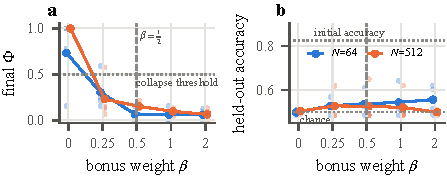
\includegraphics[width=0.6\textwidth]{../figures/fig_nn_remedy.pdf}
\caption{\textbf{Marginal-entropy bonus on the plain base-90 Transformer at $\tau=2$.} Lines: mean over 4 seeds; dots: individual seeds. The dashed line marks $\beta=\tfrac12$, above which the theory predicts stability (\cref{eq:beta}). (a)~Final order parameter $\Phi$ on the training problems; runs above the dotted line count as collapsed. The bonus removes collapse for $\beta\ge\tfrac12$. (b)~Held-out accuracy stays near chance at every $\beta$, far below the base model's initial accuracy (dotted, top).}
\label{fig:nnremedy}
\end{figure}

Without the bonus $7/8$ runs collapse, at $\beta=0.25$ $2/8$ do, and for $\beta\in\{0.5,1,2\}$ none of 24 do, matching the predicted threshold $\beta_c\le\tfrac12$ of \cref{eq:beta}.
The bonus does not, however, rescue accuracy. Remedied runs end with balanced answers ($\Phi\approx0.1$) and high confidence ($\langle|z|\rangle\approx7$), but at chance accuracy, and the learned labelling agrees with no simple input feature better than $58\%$.
The kernel explains this as well. Besides the uniform mode (eigenvalue $1.45\times10^4$), the initial kernel has several collective modes orthogonal to both the uniform direction and the current predictions, with eigenvalues $5.1\times10^3$, $2.5\times10^3$, $2.3\times10^3,\dots$, all far above the self-kernel $k_d=94$.
\Cref{prop:instab} applies to any such mode: when the uniform mode is damped, the next one takes over, and the network collapses onto a balanced but arbitrary rule.
A complete remedy must therefore damp every collective direction not aligned with the current predictions, not only the uniform one. Our analysis identifies these directions as the leading eigenvectors of the kernel restricted to that subspace.

\begin{table}[h]
\centering\small
\caption{The 22 Transformer conditions of \cref{sec:nn}. The kernel ratios and the amplification $G$ are measured on the initial network before any RL step. The base column gives the number of supervised warm-up steps and the resulting held-out accuracy. The last column counts collapsed runs out of 42 (7 values of $N$ and 6 seeds).}
\label{tab:conditions}
\begin{tabular}{llcccccc}
\toprule
model & base (acc.) & $\tau$ & $\rho_b$ & $k_u/k_d'$ & $k_s/k_d'$ & $G$ & collapsed \\
\midrule
plain & 90 (82\%) & 1 & -- & 0.702 & 0.051 & 0.025 & 29/42 \\
plain & 90 (82\%) & 2 & -- & 0.702 & 0.051 & 0.315 & 34/42 \\
plain & 90 (82\%) & 3 & -- & 0.702 & 0.051 & 0.622 & 37/42 \\
\addlinespace
plain & 120 (89\%) & 1 & -- & 0.404 & 0.058 & 0.000 & 17/42 \\
plain & 120 (89\%) & 2 & -- & 0.404 & 0.058 & 0.028 & 35/42 \\
plain & 120 (89\%) & 3 & -- & 0.404 & 0.058 & 0.186 & 38/42 \\
\addlinespace
antisymmetric & 10 (84\%) & 1 & 0 & 0.001 & 0.156 & 0.532 & 0/42 \\
antisymmetric & 10 (84\%) & 1 & 0.3 & 0.349 & 0.158 & 0.532 & 32/42 \\
antisymmetric & 10 (84\%) & 1 & 1 & 1.164 & 0.161 & 0.532 & 42/42 \\
antisymmetric & 10 (84\%) & 1 & 3 & 3.521 & 0.171 & 0.532 & 42/42 \\
antisymmetric & 10 (84\%) & 2 & 0 & 0.001 & 0.156 & 1.125 & 0/42 \\
antisymmetric & 10 (84\%) & 2 & 0.3 & 0.349 & 0.158 & 1.125 & 41/42 \\
antisymmetric & 10 (84\%) & 2 & 1 & 1.164 & 0.161 & 1.125 & 42/42 \\
antisymmetric & 10 (84\%) & 2 & 3 & 3.521 & 0.171 & 1.125 & 42/42 \\
\addlinespace
antisymmetric & 20 (92\%) & 1 & 0 & 0.002 & 0.446 & 0.177 & 0/42 \\
antisymmetric & 20 (92\%) & 1 & 0.3 & 0.436 & 0.446 & 0.177 & 22/42 \\
antisymmetric & 20 (92\%) & 1 & 1 & 1.451 & 0.447 & 0.177 & 41/42 \\
antisymmetric & 20 (92\%) & 1 & 3 & 4.361 & 0.451 & 0.177 & 42/42 \\
antisymmetric & 20 (92\%) & 2 & 0 & 0.002 & 0.446 & 0.520 & 0/42 \\
antisymmetric & 20 (92\%) & 2 & 0.3 & 0.436 & 0.446 & 0.520 & 37/42 \\
antisymmetric & 20 (92\%) & 2 & 1 & 1.451 & 0.447 & 0.520 & 42/42 \\
antisymmetric & 20 (92\%) & 2 & 3 & 4.361 & 0.451 & 0.520 & 42/42 \\
\bottomrule
\end{tabular}
\end{table}

\begin{table}[h]
\centering\small
\caption{Kernel drift during label-free RL (one seed per case). Ratios are reported only before collapse ($\Phi<0.5$): once all answers agree, $s\propto\mathbf 1$ and the decomposition degenerates. $k_d(t)/k_d(0)$ is the growth of the self-kernel, i.e.\ of the effective step size.}
\label{tab:drift}
\begin{tabular}{lrcccc}
\toprule
case & epoch & $k_u/k_d'$ & $k_s/k_d'$ & $k_d(t)/k_d(0)$ & $\Phi$ \\
\midrule
antisym 10, $\tau$=1, $\rho_b$=0.3, $N$=1024 & 0 & 0.345 & 0.152 & 1.0 & 0.02 \\
 & 1 & 0.009 & 0.222 & 28.1 & 0.28 \\
 & 4 & 0.002 & 0.074 & 101.9 & 0.14 \\
\addlinespace
antisym 20, $\tau$=1, $\rho_b$=0.3, $N$=2048 & 0 & 0.429 & 0.423 & 1.0 & 0.02 \\
 & 1 & 0.219 & 0.066 & 1.4 & 0.21 \\
 & 4 & 0.121 & 0.051 & 2.2 & 0.33 \\
 & 8 & 0.082 & 0.043 & 3.3 & 0.32 \\
\addlinespace
plain 90, $\tau$=1, $N$=512 & 0 & 0.700 & 0.050 & 1.0 & 0.04 \\
 & 1 & 0.683 & 0.092 & 1.1 & 0.25 \\
\addlinespace
plain 120, $\tau$=1, $N$=1024 & 0 & 0.405 & 0.059 & 1.0 & 0.14 \\
 & 1 & 0.384 & 0.056 & 1.2 & 0.04 \\
 & 4 & 0.304 & 0.044 & 1.6 & 0.16 \\
 & 8 & 0.254 & 0.037 & 2.2 & 0.12 \\
\addlinespace
antisym 10, $\tau$=1, $\rho_b$=0, $N$=1024 & 0 & 0.000 & 0.153 & 1.0 & 0.02 \\
 & 1 & 0.000 & 0.215 & 46.3 & 0.03 \\
 & 4 & 0.001 & 0.133 & 245.2 & 0.02 \\
 & 8 & -0.001 & 0.236 & 186.1 & 0.05 \\
\addlinespace
\bottomrule
\end{tabular}
\end{table}


\section{Experimental Details}
\label{app:details}

\paragraph{Solvable model.}
All simulations use the vectorized simulator in \texttt{src/rlvr\_collapse/sim.py}, which runs 16--24 independent seeds in parallel.
Each optimizer step draws $B$ problems without replacement (a fresh permutation each epoch), samples $K$ answers per problem from $\sigma(z_i)$ (or the softmax for $M>2$), breaks majority ties uniformly at random, and applies the chosen advantage.
Each step moves $u_i$ by $\eta\hat g_i/B$ and $v$ by $\eta\lambda\sum_i\hat g_i/B$, where $\hat g_i$ is the per-problem estimate of $F(z_i)$ (\cref{sec:theory}).
\Cref{tab:hparams} lists the settings for every sweep.
$N_c$ is obtained by maximum-likelihood fitting of $P(\text{collapse})=\sigma(k(\ln N-\ln N_c))$ to the binomial counts.
The mean-field and theory computations are in \texttt{theory.py} and \texttt{multiclass.py}.

\begin{table}[h]
\centering\small
\caption{Simulation settings. Unless listed, $K{=}3$, REINFORCE, $B{=}32$, SGD step $\eta{=}4$, 300 epochs, 24 seeds, and $80\%$ of initial majorities correct.}
\label{tab:hparams}
\begin{tabular}{lll}
\toprule
Sweep & Varied & Notes \\
\midrule
coupling & $\lambda\in\{0.035,\dots,0.28\}$, 9 values of $N$ each & $a=0.5$ \\
confidence & $a\in\{0.15,0.3,0.5,0.8,1.1,1.25\}$ & $\lambda=0.1$, $N\le32768$ \\
batch, fixed step & $B\in\{8,16,32,128,512\}$ & epochs $=300B/32$ (equal step count) \\
batch, linear scaling & $B\in\{8,\dots,512\}$ & $\eta=4B/32$, 300 epochs \\
long training & $a\in\{1.4,1.6,2.0\}$, $\lambda\in\{0.1,0.3\}$ & 3000 epochs (600 at $N=16384$); 16 seeds \\
heterogeneous & 7 initial distributions & $\lambda=0.1$ \\
feature coupling & $\mu\in\{0,\dots,0.07\}$, $N\in[128,32768]$ & $\lambda=0.1$, 16 seeds \\
remedy & $\beta\in\{0,0.1,0.25,0.5,1,2\}$, $a\in\{0.2,0.5\}$ & $\lambda=0.1$, 16 seeds \\
GRPO / $K$ & $K\in\{3,5,8,16\}$; GRPO, mean baseline, REINFORCE & step set so that $\eta F^\star_K\in[0.38,0.48]$ \\
many answers & $(M,K)\in\{(3,3),(4,5),(6,5)\}$ & softmax logits, vector $v$ \\
Adam & $\lambda\in\{0.2,\dots,1.0\}$, $N\in[64,16384]$ & lr $0.01$, $(\beta_1,\beta_2)=(0.9,0.999)$, 16 seeds \\
\bottomrule
\end{tabular}
\end{table}

\paragraph{Transformer.}
Embedding width 64, 2 pre-LN encoder layers, 4 heads, MLP width 256, no dropout, a learned positional embedding and a CLS token. The readout is a bias-free linear map to the logit difference, plus the optional scaled scalar bias $\lambda_bb$.
Supervised warm-up uses Adam (lr $10^{-3}$, batch 128) on fresh labeled samples.
RL uses the first $N$ problems of a fixed pool of 8192 unlabeled problems, plain SGD with step $0.125B/k_d$ (where $k_d$ is the mean self-kernel at the given temperature), $B=16$, $K=3$, REINFORCE with majority-vote rewards, and 100 epochs.
Accuracy is measured on 2000 held-out problems.
Per-example gradients for the kernel statistics are computed with \texttt{torch.func} on 384 pool problems.
The amplification $G$ is computed from the initial logits of 2048 pool problems.
A run counts as collapsed if $|\langle\mathrm{sign}\,z\rangle|>0.5$ on its training problems at the end of training.

\paragraph{Compute.}
All experiments ran on a single Apple M4 Pro CPU (14 cores).
The full solvable-model study takes under an hour, and the 924 Transformer runs take about 40 minutes.
